\documentclass[journal,10pt,twocolumn]{article}
\usepackage{graphicx}
\graphicspath{{./Figures/}}
\usepackage[margin=0.5in]{geometry}
\usepackage[cmex10]{amsmath}
\usepackage{amssymb}
\usepackage{array}
\usepackage{booktabs}
\title{\textbf{Conic Assignment}}
\author{Bole Manideep}
\date{September 2022}

\providecommand{\norm}[1]{\left\lVert#1\right\rVert}
\providecommand{\abs}[1]{\left\vert#1\right\vert}
\let\vec\mathbf
\newcommand{\myvec}[1]{\ensuremath{\begin{pmatrix}#1\end{pmatrix}}}
\newcommand{\mydet}[1]{\ensuremath{\begin{vmatrix}#1\end{vmatrix}}}
\providecommand{\brak}[1]{\ensuremath{\left(#1\right)}}

\begin{document}

\maketitle
\paragraph{\textit{Problem Statement} -Find the radius of the circle passing through the foci of the elipse $\frac{\hspace{1mm}x^2}{16} + \frac{\hspace{1mm}y^2}{9} =1$ and having its centre at (0,3)}

\section*{Solution}

\begin{figure}[h]
\centering
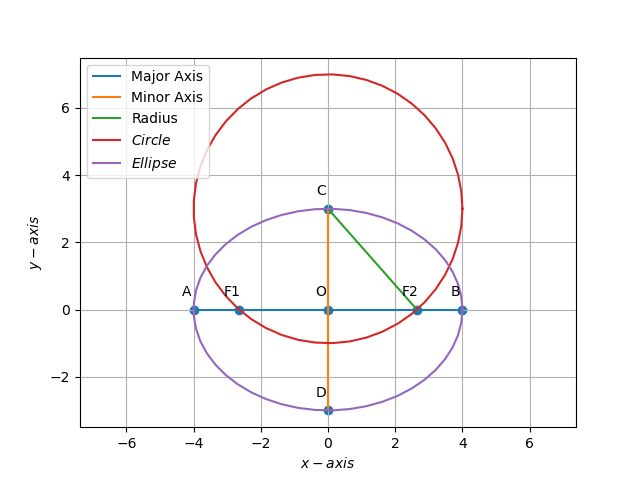
\includegraphics[width=1\columnwidth]{Question.png}
\caption{Ellpise with center O along with Circle C}
\label{fig:Ellipse}
\end{figure}


\raggedright Given an ellipse with center $\vec{O}$ and semi major axis lenth a = 4cm and semi  minor axis length b = 3cm. \vspace{2mm}
\\Let $\vec{F_1} \hspace{1mm} \& \hspace{1mm} \vec{F_2}$ be the Focii of the ellipse, where $\vec{A},\vec{B} \hspace{2mm} \& \hspace{2mm} \vec{C},\vec{D}$ be the extreme points on major $\&$ minor axis respectively. \vspace{2mm}
\\The equation of a conic with diretrix $\vec{n}^{\top}\vec{x} = c$, eccentricity e and Focus $\vec{F}$ is given by,
\begin{equation}
\vec{x}^{\top}\vec{V}\vec{x}+2\vec{u}^{\top}\vec{x}+f=0
\label{eq-1-}
\end{equation}
For the given equation of ellipse,
\begin{equation}
\vec{V} = \begin{pmatrix} 
	9 & 0 \\
	0 & 16 \\
	\end{pmatrix}, \hspace{4mm} \vec{u} = \myvec{0 \\ 0} \hspace{2mm} \& \hspace{2mm} f = -144
\label{eq-2-}
\end{equation}
The eigenvalue decomposition of a symmetric matrix $\vec{V}$ is given by
\begin{equation}
\vec{P}^{\top}\vec{V}\vec{P} = \vec{D} \hspace{1cm} 
\vec{P} = \myvec{\vec{P_1} & \vec{P_2}} 
\label{eq-3-}
\end{equation}
\begin{equation}
\vec{D} = \begin{pmatrix} 
	\lambda_1 & 0 \\
	0 & \lambda_2 \\
	\end{pmatrix} 
\label{eq-4-}
\end{equation}
On solving $\eqref{eq-3-}$ with $\vec{P_1} = \myvec{1 \\ 0} \hspace{2mm} \& \hspace{2mm} \vec{P_2} = \myvec{0 \\ 1}$, we get
\begin{equation}
\vec{D} = \begin{pmatrix} 
	9 & 0 \\
	0 & 16 \\
	\end{pmatrix}
\label{eq-5-}
\end{equation}
where,
\begin{equation}
\lambda_1 = 9 \hspace{2mm} and \hspace{2mm} \lambda_2 = 16
\label{eq-6-}
\end{equation}
We have,
\begin{equation}
eccentricity, \hspace{3mm} e = \sqrt{1-\frac{\lambda_1}{\lambda_2}}
\label{eq-7-}
\end{equation}
from \eqref{eq-6-},
\begin{equation}
e = 0.6614
\label{eq-8-}
\end{equation}
Normal vector of diretrix $\vec{n}$ is given by
\begin{equation}
\vec{n} = \sqrt{\lambda_2}\vec{P_1}
\label{eq-9-}
\end{equation}
This gives,
\begin{equation}
\vec{n} = \myvec{4 \\ 0}
\label{eq-10-}
\end{equation}
For e $\neq$ 1, we have
\begin{equation}
c = \frac{e\vec{u}^{\top} \vec{n}\pm \sqrt{e^2\brak{\vec{u}^{\top}\vec{n}}^2 - \lambda_2 \brak{e^2-1}\brak{\norm{\vec{u}}^2-\lambda_2 f }}}{\lambda_2 e \brak{e^2-1}}
\label{eq-11-}
\end{equation}
On solving we get,
\begin{equation}
c = \pm 24.1911
\label{eq-12-}
\end{equation}
Focii of a conic is given by the equation,
\begin{equation}
\vec{F} = \frac{ce^2\vec{n}-\vec{u}}{\lambda_2}
\label{eq-13-}
\end{equation}
Yelding,
\begin{equation}
\vec{F} = \pm 2.6456
\label{eq-14-}
\end{equation}
Therefore, focii of the ellipse are,
\begin{equation}
\vec{F_1} = \myvec{-2.6456 \\ 0} \hspace{2mm} \& \hspace{2mm} \vec{F_2} = \myvec{2.6456 \\ 0}
\label{eq-15-}
\end{equation}
Given $\vec{C} = \myvec{0 \\ 3}$ is the center of the circle and is passing through focii of the ellipse.\\
Let the circle be,
\begin{equation}
\vec{x}^{\top}\vec{V}\vec{x}+2\vec{u_1}^{\top}\vec{x}+f_1=0
\label{eq-16-}
\end{equation}
where, 
\begin{equation}
\vec{V} = \vec{I} \hspace{4mm} \& \hspace{4mm} \vec{u_1} = \myvec{0 \\ -3}
\end{equation}
Since circle is passing through $\vec{F_1}$
\begin{equation}
\vec{F_1}^{\top}\vec{V}\vec{F_1}+2\vec{u_1}^{\top}\vec{F_1}+f_1=0 
\label{eq-18-}
\end{equation} \vspace{1mm}
\begin{equation}
\myvec{-2.6456 & 0} \myvec{-2.6456 \\ 0} +  2\myvec{0 & -3}\myvec{-2.6456 \\ 0} +  f_1 = 0 
\end{equation}
\begin{gather*}
6.99 + 0 +  f_1 = 0 \\
\implies f_1 = -6.99
\end{gather*}
Hence, Equation of the circle is given as,
\begin{equation}
\vec{x}^{\top}\vec{I}\vec{x}+2\myvec{0 \\ -3}\vec{x}-6.99=0
\label{eq-20-}
\end{equation}
We have, radius of the circle,
\begin{equation}
r = \sqrt{\norm{\vec{u}}^2-f_1}
\label{eq-21-}
\end{equation}
\begin{gather*}
r = \sqrt{\brak{\sqrt{0^2 + (-3)^2}}^2-(-6.99)} \\
r = \sqrt{9+6.99} \\
r = \sqrt{15.99}
\end{gather*}
\begin{equation}
\therefore \hspace{3mm} Radius, r = 3.99 cm
\label{eq-22-}
\end{equation}


\section*{Construction}
\raggedright An ellipse with center O and major,minor axis a,b respectively along with circle with center C is constructed unsing python,with the parameters that are mentioned in the table below.
\vspace{5mm}
\begin{center}
    \setlength{\arrayrulewidth}{0.1mm}
	\setlength{\tabcolsep}{10pt}
	\renewcommand{\arraystretch}{1.5}
\begin{tabular}{|c|c|c|}
	\hline 
    \textbf{Symbol} & \textbf{Value} & \textbf{Description}\\ 		\hline
    a & 4 & Semi Major Axis \\ \hline
    b & 3 & Semi Minor Axis \\ \hline
    $\vec{O}$ & $\myvec{0 \\ 0}$ & Center of Ellipse \\ \hline
    $\vec{e1}$ & $\myvec{1 \\ 0}$ & Unit Vector along x-axis \\ 		\hline
    $\vec{e2}$ & $\myvec{1 \\ 0}$ & Unit Vector along y-axis\\ 			\hline
    $\vec{A}$ & -a$\ast\vec{e1}$ & Vertex A \\ \hline
    $\vec{B}$ & a$\ast\vec{e1}$ & Vertex B \\ \hline
    $\vec{C}$ & b$\ast\vec{e2}$ & Center of circle (C) \\ \hline
    $\vec{D}$ & -b$\ast\vec{e2}$ & Vertex D \\ \hline
    d & $\sqrt{a^2 - b^2}$ & distance between Center (O) \& Focii 	\\ \hline
    $\vec{F_1}$ & -d$\ast$e1 & Focus 1 of Ellipse \\ \hline
    $\vec{F_2}$ & d$\ast$e1 & Focus 2 of Ellipse \\ \hline
\end{tabular}\\ \vspace{2mm}
Table 1: Parameter's Table
\end{center}

\end{document}